% Cross-Era Fantasy Cricket - final report.
% No course template was found in docs/report/template/, so this is a plain two-column article.
% Hard limit: 4 pages INCLUDING references. Compile: pdflatex main && bibtex main && pdflatex main && pdflatex main
\documentclass[10pt,twocolumn]{article}
\usepackage[a4paper,margin=0.7in,columnsep=0.25in]{geometry}
\usepackage{graphicx,booktabs,amsmath,url,microtype}
\usepackage[hidelinks]{hyperref}
\usepackage[font=small,labelfont=bf]{caption}
\setlength{\textfloatsep}{8pt plus 2pt minus 2pt}
\setlength{\floatsep}{6pt plus 2pt minus 2pt}
\setlength{\abovecaptionskip}{3pt}

\title{\vspace{-1.5em}Cross-Era Fantasy Cricket: Animating Historical Cricketers\\with Modern Motion on Free Hardware\vspace{-0.5em}}
\author{[TODO: team member names, IDs] \quad Course: [TODO: course code and name]}
\date{\vspace{-1.5em}}

\begin{document}
\maketitle

\begin{abstract}
We animate historical cricketers from a single archival photograph using motion taken from modern broadcast footage, and
render the result in the visual style of the player's era. Our pipeline extracts whole-body pose with DWPose on a laptop
CPU, builds a control video (pose skeleton or depth), generates the clip with Wan2.1-VACE-1.3B in a headless ComfyUI
running on a free Kaggle T4 GPU, retimes it to real speed and applies 1930s/1970s/1990s era filters. A $2{\times}2$
ablation (control type $\times$ reference crop) plus a seed sweep shows that a depth control fixes the most visible
failure of skeleton control, a missing or wrong bat, and lowers brightness flicker, while a tighter reference crop does
not clearly improve likeness and seed variation dominates the reference effect. All outputs are labelled
``AI-generated -- academic project''.
\end{abstract}

\section{Introduction}
``Fantasy cricket'' across eras is usually a statistical exercise. We ask what such a match could \emph{look} like: Sir Don
Bradman playing a modern cover drive, or Harold Larwood bowling a modern delivery. The task is reference-guided human
image animation: one photograph supplies the appearance, and a driving video supplies the motion. Cricket makes it hard:
fast limb motion, a thin bat that the skeleton does not describe, other people in frame, and archival references that are
black-and-white, low resolution and often half-body.

Our constraints were strict: a laptop with a 6\,GB RTX 4050 and 16\,GB RAM, no paid GPUs, and a short deadline. Our
contributions are: (i) a reproducible, free pipeline (laptop CPU + Kaggle T4) from broadcast clip to styled video;
(ii) a depth-control variant, with a \emph{target-only} mode that removes other people, which fixes bat
preservation; (iii) a controlled ablation with an honest negative result on reference cropping; and (iv) era styling
and real-speed retiming for presentation-quality output.

\section{Related Work}
\textbf{Pose estimation.} DWPose~\cite{yang2023dwpose} distils RTMPose-style models~\cite{jiang2023rtmpose} into a
133-keypoint whole-body estimator. Its OpenPose-style renderings are the de-facto control input for human animation.
\textbf{Human image animation.} Animate Anyone~\cite{hu2023animateanyone} and MagicAnimate~\cite{xu2023magicanimate}
add a reference/appearance branch to Stable Diffusion with pose or DensePose guidance. AnimateDiff~\cite{guo2023animatediff}
adds a motion module to text-to-image models. MimicMotion~\cite{zhang2024mimicmotion} uses confidence-aware pose guidance
on Stable Video Diffusion. The project proposal named LTX-2~\cite{ltx2} and MagicAnimate. We found that LTX-2 conditions on
the reference only as a first frame and targets 32\,GB+ GPUs, and that MagicAnimate's released code is old (SD1.5) and
DensePose-based, so we kept MagicAnimate/AnimateDiff as the team's baseline engine.
\textbf{Video diffusion transformers.} Wan2.1~\cite{wan2025} is an open video DiT family. VACE~\cite{jiang2025vace}
adds unified conditioning (reference images, pose, depth, masks); its 1.3B variant fits a free T4.
\textbf{Depth and features.} Depth Anything V2~\cite{yang2024depthanythingv2} gives robust monocular relative depth.
DINOv2~\cite{oquab2023dinov2} provides general image features, which we use for an identity proxy.
U$^2$-Net~\cite{qin2020u2net} (via rembg) removes reference backgrounds.

\begin{figure*}[t]
  \centering
  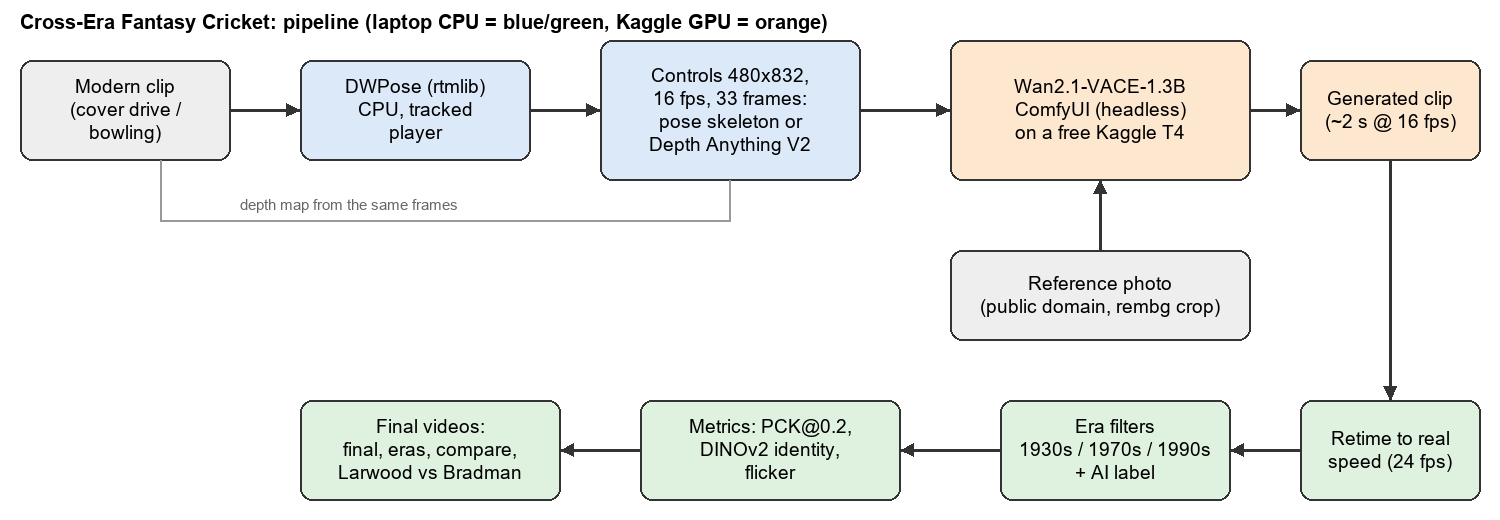
\includegraphics[width=0.74\textwidth]{figs/pipeline.png}
  \caption{Pipeline. Laptop CPU stages in blue/green, the Kaggle T4 stage in orange.}
  \label{fig:pipeline}
\end{figure*}

\section{Method}
\textbf{Motion extraction.} We run rtmlib's YOLOX detector and DWPose-l ($384{\times}288$) on CPU. The target player is
selected by a box on frame~0 and followed by best-IoU tracking, because broadcast frames also contain the umpire,
non-striker or fielders. Keypoints below confidence 0.3 are masked, gaps of up to 4 frames interpolated, and trajectories
smoothed (Savitzky--Golay, window 7). We resample to exactly 33 frames at 16\,fps and place the player on a
$480{\times}832$ portrait canvas with one global scale and offset, so the body fills ${\sim}85\%$ of the height. An 8\% top
margin, whose box includes an estimated head top, the feet and the fingers, keeps the head and a raised bowling hand in frame.

\textbf{Controls.} \emph{Skeleton}: an OpenPose-style render (body, hands, face) on black. \emph{Depth}: Depth Anything
V2 Small on the same source frames, warped with the \emph{same} affine as the skeleton, so the two line up frame by frame.
Depth is normalised with one global min/max over the clip (no per-frame stretch, no flicker), with near = bright. The head
region is flattened inside the silhouette, so a modern helmet's grille does not override the reference face.
\emph{Target-only} (bowler clip): a person mask around the tracked box (rembg), restricted to blobs containing the
player's keypoints and to a capsule around his skeleton, keeps only the bowler. Fielders' legs become flat background.

\textbf{Reference.} rembg removes the background, the player is placed on white, and the crop fills ${\sim}90\%$ of the
canvas with the head near the top. This is the \emph{tight crop}; the \emph{padded} reference is the photo letterboxed
into the canvas.

\textbf{Generation.} Wan2.1-VACE-1.3B (fp16 DiT, fp8 UMT5 text encoder) runs in ComfyUI driven headlessly through its
API on a Kaggle T4 (no bf16, so fp16 with an fp32 VAE): 20 steps, CFG 5, \texttt{uni\_pc}, shift 8, seed 42 unless
stated. A 17-frame run takes ${\approx}$270\,s and a 33-frame run ${\approx}$520\,s with a 12.8--14.9\,GB peak, far
beyond the 6\,GB laptop GPU. Three Kaggle-specific bugs (dependency filtering, dataset mount depth,
input previews listed as outputs) were fixed in the notebook. The prompt describes 1930s kit; the negative prompt lists
failure modes (extra balls, two bats, modern logos; for the bowler also bat, hat, suit and cigarette).

\textbf{Post-processing.} The batter's 33 frames cover 5.6\,s of source, so they play $2.7{\times}$ too fast at 16\,fps.
We retime to real speed at 24\,fps. Frame blending (ffmpeg \texttt{framerate}) was chosen over motion-compensated
interpolation (\texttt{minterpolate}), which tore the thin bat and drifted in timing. The 2.0\,s bowler clip is sampled at
real speed and shown in $2{\times}$ slow motion with frame holds (blending ghosted at that factor). Seeded OpenCV era
filters (Table~\ref{tab:eras}) keep the duration and burn an ``AI-generated'' label into every frame. Bowler and batter
can be styled in different eras for a cross-era match.

\section{Experiments}
\textbf{Metrics} (CPU). \emph{PCK@0.2}: DWPose is re-run on the output and the 17 body joints are compared with the
control keypoints (threshold $0.2\times$ torso length). \emph{Identity}: cosine similarity of DINOv2-small CLS embeddings
between grayscale person crops of each frame and of the tight (``crop'') or original (``orig'') reference.
\emph{Flicker}: standard deviation of per-frame mean brightness, and mean absolute frame difference.

\textbf{Ablation.} $2{\times}2$ over control (skeleton / depth) and reference (padded / tight crop), all 17 frames, seed
42: A (skeleton, padded; older prompt, no margin), B (depth, padded), C (skeleton, crop), D1 (depth, crop). D1--D4 repeat
D1's inputs with seeds 42/7/123/2024 to measure seed variance. B vs D1 isolates the reference, and C vs D1 the control.
\textbf{Finals.} 33-frame depth + crop runs with the default prompt (F1, cap) and a bare-headed prompt (F2).
\textbf{Bowler.} L1--L3: target-only depth + Larwood crop, seeds 42/7/2024, 33 frames (real speed; shown at
$2{\times}$ slow motion). \textbf{Era filters.} Each preset is applied to the raw F1 and L3 clips at native timing; besides
PCK and identity we report a Farneback warping error (luminance error after warping frame $t$ onto $t{+}1$ where
forward/backward flow agree; lower = smoother).

\section{Results}
\begin{table}[t]
\centering\small
\setlength{\tabcolsep}{3.2pt}
\begin{tabular}{lllccccc}
\toprule
Run & Ctrl & Ref & PCK & ID$_\text{crop}$ & ID$_\text{orig}$ & B.std & F.diff\\
\midrule
A  & skel  & pad  & 0.934 & 0.205 & 0.158 & 2.27 & 10.10\\
B  & depth & pad  & 0.997 & 0.223 & 0.291 & 1.63 & 11.43\\
C  & skel  & crop & 0.969 & 0.172 & 0.130 & 2.49 & 10.62\\
D1 & depth & crop & 0.983 & 0.206 & 0.207 & 1.98 & 10.26\\
D2 & depth & crop & 0.900 & 0.230 & 0.227 & 1.49 & 10.97\\
D3 & depth & crop & 0.979 & 0.165 & 0.156 & 2.06 & 11.90\\
D4 & depth & crop & 0.990 & 0.302 & 0.305 & 1.25 & 10.40\\
\midrule
F1 & depth & crop & 0.904 & 0.217 & 0.175 & 1.65 & 11.93\\
F2 & depth & crop & 0.882 & 0.203 & 0.195 & 3.78 & 9.17\\
\midrule
L1 & depth$^\dagger$ & crop & 0.788 & 0.124 & 0.108 & 4.26 & 12.17\\
L2 & depth$^\dagger$ & crop & 0.851 & 0.092 & 0.102 & 4.93 & 15.42\\
L3 & depth$^\dagger$ & crop & 0.801 & 0.125 & 0.086 & 1.81 & 11.06\\
\bottomrule
\end{tabular}
\caption{Ablation (17 frames; F1/F2 and L: 33 frames). D1--D4 differ only in seed (42/7/123/2024); L1--L3 seeds 42/7/2024.
$^\dagger$target-only depth. Identity for L1--L3 is measured against Larwood.}
\label{tab:ablation}
\end{table}

\begin{figure*}[t]
  \centering
  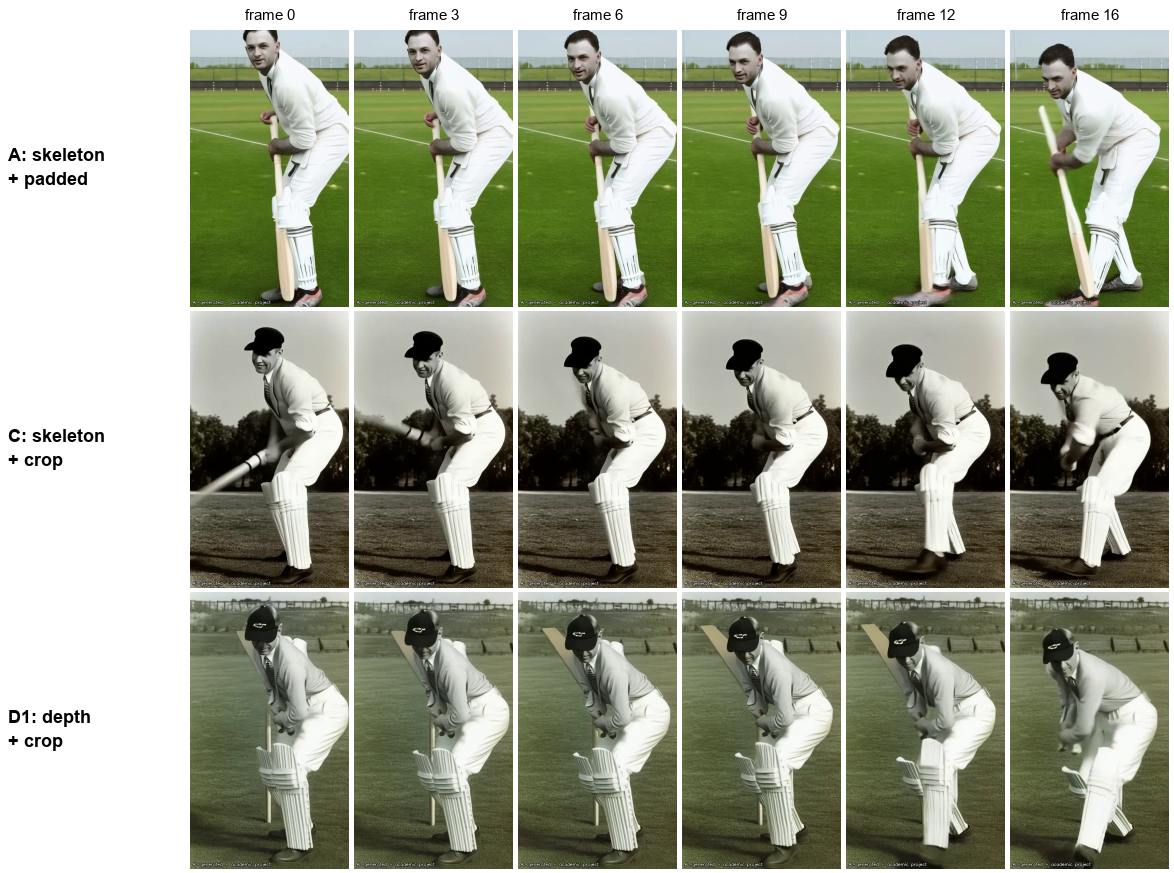
\includegraphics[width=0.62\textwidth]{figs/ablation_strip.png}
  \caption{Ablation outputs (raw, 17 frames). With the skeleton (A, C) the bat is lost or wrong; with depth (D1) one bat
  is held for the whole clip. A dark cap hides the face in the crop runs.}
  \label{fig:ablation}
\end{figure*}

\textbf{Depth fixed the bat.} By visual inspection, every depth run (B, D1--D4) holds one proper bat for the whole clip,
with the head in frame and no extra balls. Both skeleton runs (A, C) lose the bat (Fig.~\ref{fig:ablation}). The skeleton
simply carries no bat information. Motion fidelity stays high for all runs (PCK 0.90--1.00, Table~\ref{tab:ablation}), so
depth costs no motion accuracy.
\textbf{Flicker.} Depth lowered brightness flicker (mean brightness std 2.38 for the skeleton runs vs 1.68 for depth).
Mean frame difference did \emph{not} drop (10.36 vs 10.99), plausibly because the depth runs swing the bat through a
fuller arc.
\textbf{Reference crop: no clear gain.} With control and seed fixed, padded$\rightarrow$crop changes identity by
$-0.017$ (vs crop) and $-0.084$ (vs original) for depth (B$\rightarrow$D1), and by $-0.034$ for the skeleton
(A$\rightarrow$C). A likely cause is the dark cap that hides the face in the crop runs.
\textbf{Seed dominates.} Across D1--D4 identity spans 0.137 (crop) and 0.149 (orig), several times the reference effect.
Single-seed likeness comparisons are therefore inconclusive; the bat result is not, since it held in 5/5 depth runs and
failed in 2/2 skeleton runs. D3/D4 also drifted to modern dark pads.
\textbf{Finals.} F1 and F2 are close numerically (Table~\ref{tab:ablation}). We chose \textbf{F1 (cap)} by visual
inspection, for its better face and cleaner bat (Fig.~\ref{fig:final}).
\textbf{Bowler.} All three runs are bare-headed with no fedora, cigarette or suit (the negative prompt overrode the
reference clothing), show no extra people (target-only depth removed the fielders) and no bat. L1 has the cleanest
release but a grey short-sleeved shirt; L2 the clearest face, but the ball smears (highest frame difference); L3 a
knitted cardigan, the most 1930s kit, and the lowest flicker. We chose \textbf{L3}, shown at $2{\times}$ slow motion.
PCK is lower than for the batter (0.79--0.85) because the overarm action is the fastest, most blurred motion.
\textbf{Era filters} (Table~\ref{tab:eras}, Fig.~\ref{fig:eras}) keep the motion: the batter's PCK drops by at most
0.08 (0.007 for 1990s), the fast bowling arm by up to 0.12. The 1930s look deliberately adds flicker and texture
(brightness std ${\approx}2.5{\times}$, warping error ${\approx}1.7{-}2.9{\times}$), while the softer 1970s/1990s filters
slightly lower the warping error. In the cross-era match, Larwood bowls in 1930s film and Bradman drives in 1990s broadcast.

% PAGE BUDGET: if the PDF exceeds 4 pages, delete this figure first (its content is also in the video),
% then shrink figs/ablation_strip.png further.
\begin{figure}[t]
  \centering
  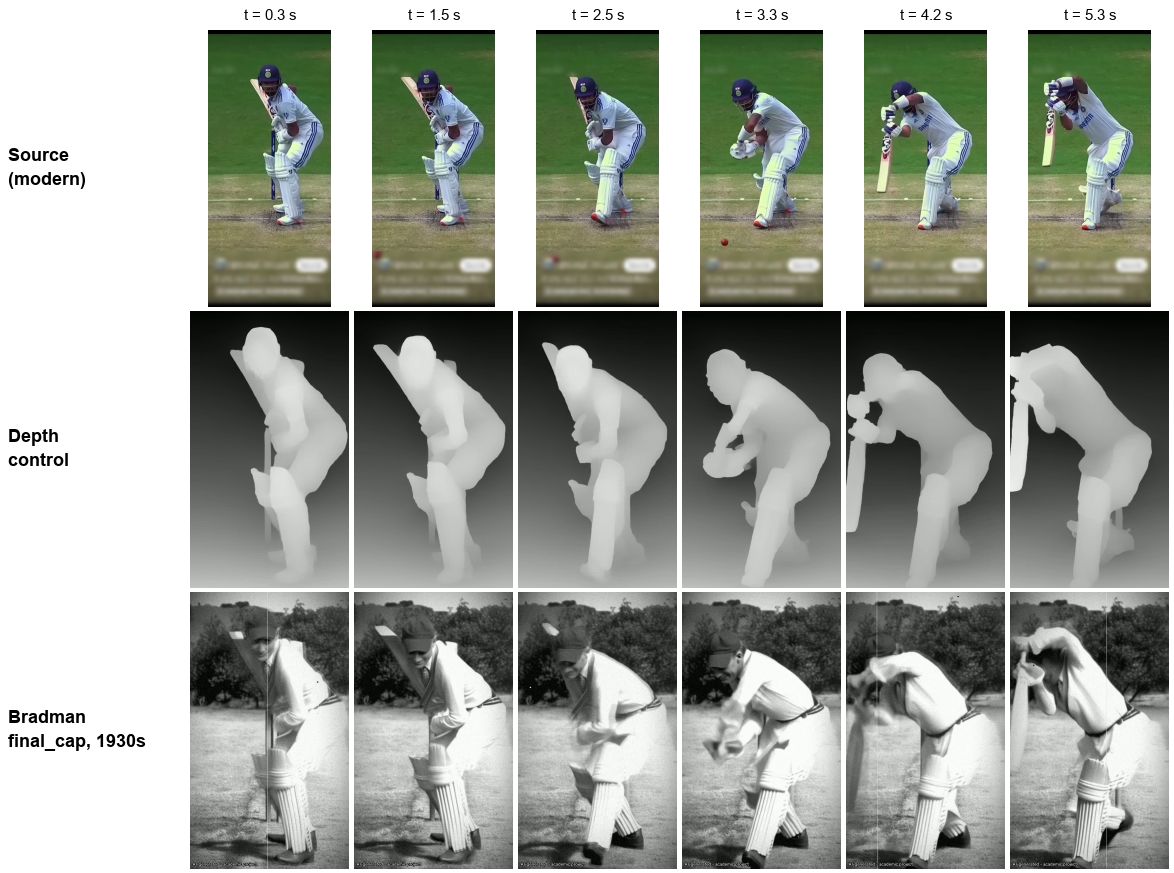
\includegraphics[width=\columnwidth]{figs/final_strip.png}
  \caption{Final batter clip on the source timeline: source (overlays blurred), depth control, F1 in 1930s style.}
  \label{fig:final}
\end{figure}

\begin{table}[t]
\centering\small
\setlength{\tabcolsep}{2.6pt}
\begin{tabular}{llcc}
\toprule
Preset & Look & PCK bat/bowl & Warp bat/bowl\\
\midrule
raw & VACE output, 16\,fps & 0.904 / 0.801 & 5.72 / 3.40\\
1930s film & 18\,fps uneven, gray, grain, weave, & 0.870 / 0.698 & 9.81 / 9.91\\
 & flicker, dust, scratches, vignette & & \\
1970s TV & 25\,fps, desat., warm, chrom. aberr., & 0.829 / 0.684 & 4.06 / 3.08\\
 & scanlines, tape noise, bloom & & \\
1990s bcast & 25\,fps, mild colour, chroma bleed, soft & 0.897 / 0.774 & 3.27 / 2.65\\
\bottomrule
\end{tabular}
\caption{Era presets and their effect on Bradman F1 / Larwood L3 (raw clip styled at native timing).}
\label{tab:eras}
\end{table}

\begin{figure}[t]
  \centering
  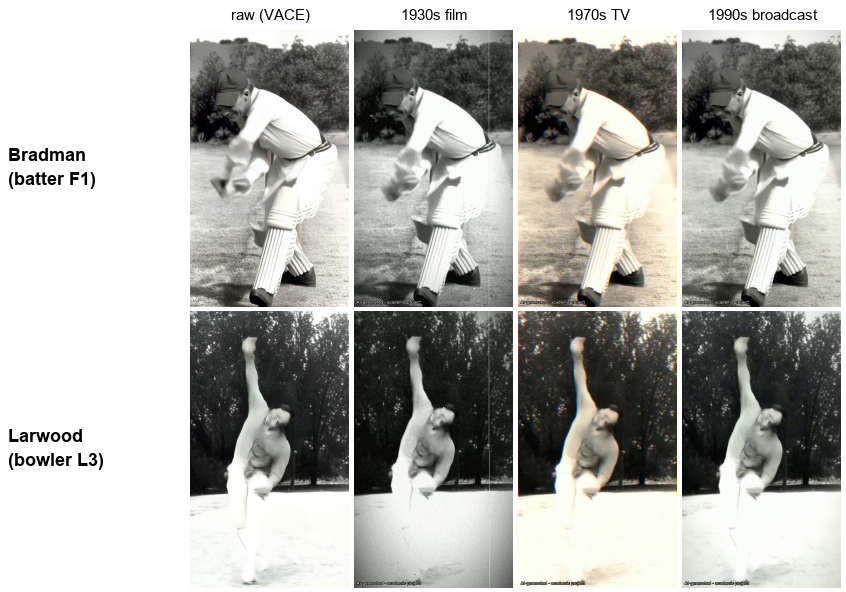
\includegraphics[width=\columnwidth]{figs/era_strip.png}
  \caption{The same moment raw and in the three era styles (batter F1, bowler L3).}
  \label{fig:eras}
\end{figure}

\section{Limitations and Ethics}
\textbf{Limitations.} Likeness is weak: identity scores are low in absolute terms (whole-body DINOv2 crops also measure
clothing and pose, so they rank runs rather than measure likeness). The depth map carries the modern helmet's outline,
so a dark cap often hides the face. The model copies reference clothing (Larwood's 1929 photo shows a fedora, suit and
cigarette, which we suppress only through the negative prompt). Clips are short (2--5.6\,s), single-player and
single-seed for the finals. Bowler and batter are generated separately and cut together, not as one interaction; the bowler is shown in
slow motion and L3 came out nearly monochrome, so its later-era versions differ mainly in texture.
\textbf{Ethics.} The videos depict real, deceased public figures in actions they never performed. Every generated frame
and title card carries a burned-in ``AI-generated -- academic project'' label, and the work is for academic use only.
Reference photos are public domain (Larwood: National Library of Australia, Fairfax glass plate, 1929,
nla.obj-161865715; Bradman: [TODO: source]). The modern broadcast clips are used only to extract motion, are not
redistributed, and their overlays are blurred in figures.

\section{Individual Contributions}
[TODO: confirm with team.] \textbf{Student 1} [TODO name]: pose/motion engine (tracking, DWPose, smoothing, control
renders). \textbf{Student 2} [TODO name]: AnimateDiff/MagicAnimate generation engine (team baseline).
\textbf{Student 3, Krishav}: era styling and evaluation; VACE pipeline (depth/target-only controls, Kaggle notebook,
retiming, final videos); ablation; bowler clip.

\section{Generative AI Disclosure}
We used Claude (Anthropic) to assist with background research, code (pipeline scripts and the Kaggle notebook) and
drafting this report. All code was run and tested by us, all outputs and numbers were checked against our own runs, and
the design decisions and conclusions are ours.

\textbf{Code:} \url{https://github.com/krishavgoyal/Cross_Era_Fantasy_Cricket} (branch \texttt{Krishav-main}).

\small
\bibliographystyle{ieeetr}
\bibliography{refs}
\end{document}
